\clearpage
\subsubsection{Evil Twin/Honeypot Attack}
\label{sec:honeypot}
The Evil Twin, aka Honeypot, WiFi Phishing, AP Phishing, etc., is a gateway attack leveraged to give the attacker the ability to perform other exploits. Victims leave themselves open to a whole host of MITM exploits, including HTTP cache poisoning and session hijacking, as mentioned previously, along with having secure information such as credit card information, website login credentials and personal data stolen. Particularly worrying is the coupling of a honeypot attack, and then a MITM attack that includes the use of SSLstrip \cite{research:youtube}\cite{research:benson} in an attempt to beat HTTPS. There are new protocols that have been proposed that would prevent this, such as HTTP Strict Transport Security (HSTS) \cite{research:hsts}; however, this is out of scope of this project.

The attack takes advantage of the Preferred Network List (PNL) that wireless devices maintain once successful connection with an access point has been made. When a device is not connected to a wireless network, it will broadcast probe request frames of all the previous networks it has been attached to. When attached to a network, it broadcasts probe requests for that network to allow it to roam between BSSs in an ESS. 

\begin{figure}[h!]
\centering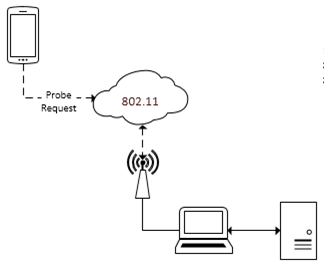
\includegraphics{research/attackvectors/figures/honeypot.png}
\caption{The smartphone sends a probe request frame which is picked up by the attacker.}
\end{figure}

The attack can be traced as far back as 2003 \cite{research:old_paper}, with the KARMA Wireless Client Security Assessment Tools \cite{research:old_toos} arriving in 2005 and making life easier, for the small percentage of people with the ability to patch drivers, by releasing patches for the Linux MadWifi driver. This application was released purely as a gateway to users writing their own exploits, termed BYOX (Bring Your Own eXploit). This set of tools was certainly ahead of its time in the security landscape, as wireless enabled devices were scarce when compared to today where not only smartphones are increasingly popular \cite{research:device_survey}, but with the advent of The Internet of Things, and the preference to use WiFi in products \cite{research:use_wifi}\cite{research:use_wifi2}, more devices are being made vulnerable to old attacks.  

To perform the attack, the attacker needs to gain the SSID of access points either through beacon packets of real access points if performing a disassociation evil twin attack, as performed in section \ref{ddos-atk}, or by probe requests broadcast by passing devices if performing the honeypot style. The honeypot style of attack differs from the Evil Twin in that it takes advantage of passing devices. 

If a real access point is the target, the attacker can disconnect users from the real access point through a deauthentication DOS and broadcast the fake access point beacon packets with a stronger signal than the real one. Passing devices sending out probe requests will connect to the access point with the strongest signal, which happens to be the fake one. If the attacker is sniffing for probe request frames to perform a honeypot, they need to perform the association sequence once a valid probe request frame is detected. This can be achieved using low-level packet injection/monitoring libraries, or through a suite of tools found in Linux penetration testing distributions.  

This attack is not thwarted by WEP or WPA, as they only encrypt data after the association is established, thus not protecting against management packet spoofing. There have been efforts made to protect against this attack, not by protecting against MAC spoofing, but by utilising the received signal strength (RSS). This proves a good method of protection for single transmitter source, and it has also been demonstrated to have a 97.8\% success rate with multiple transmitters \cite{4509834}. 802.11w does implement protected management frames and as a result would eliminate this style of attack, I touch upon this in section \ref{80211w}.

The honeypot attack forms the basis of the program this project is implementing and as such will be detailed in the implementation section of the report.